%sse
\documentclass[../../main/main.tex]{subfiles}


\begin{document}
\title{Systems Security Engineering}


%%%%%%%%%%%%%%%%%%%%% Chapter CSBD ACL %%%%%%%%%%%%%%%
\chapter{Systems Security Engineering \& Patrol Base Operations}\label{chp:sse}


       %%%%%%%%%%%%%%%%%% Section Systems %%%%%%%%%%%%%%%%
\section{The Systems Perspective}\label{sec:systems}
A system is a set of interacting and interdependent components that act as a whole to perform some behavior or function.  Examples of systems include the human body, socio-political systems, and computer systems. 

The patrol base operations satisfy this definition of a system.  As a whole, the patrol base operations perform some function(s).  This function is described in the Ranger Handbook \cite{rangermanual} and discussed in section \ref{sec:pb}.  The patrol base operations are comprised of interdependent and interacting components.  In general these components are the individual soldiers.  But, the way this master thesis defines the patrol base operations, the definition of a component varies.

This master thesis defines the patrol base operations as a system of systems.  More specifically, this thesis models the patrol base operations as a hierarchy of \glsentrylongpl{ssm}.  Chapter \ref{chp:ssmmodel} describes \glsentryshortpl{ssm} in general.   Section \ref{sec:modelingpb} describes this model of the patrol base operations.  This model presents the patrol base operations as a hierarchy wherein each level of the hierarchy represents a decreasing level of abstraction.   

At the top and most abstract level, the components are phases of the patrol base operations.  These phases commence in a sequential order to achieve the goal of the patrol base operations.  Each lower level of the hierarchy is composed of less abstract phases. At each level, the components function sequentially (typically) to achieve the ultimate goal.  

This system of system also contains non-hierarchically defined components.  For example, an escape-level component models situations wherein the patrol base operations are aborted.  The escape level component is reachable from any component at any level of the hierarchy.  Soldiers also function within this system of systems in a non-hierarchical manner.  However, soldiers were not modeled in detail for this master thesis.  Nevertheless, they were discussed in detail and ready to be modeled.

In this way, the patrol base operations represent a system and are amiable to the systems engineering perspective.  

     %%%%%%%%%%%%%%%%%% Section Systems Engineering %%%%%%%%%%
\section{Systems Engineering}\label{sec:se}
Systems engineering is an interdisciplinary approach aimed at solving problems involved in the design, development, realization, and life-cycle maintenance of systems.
  

ISO/IEC/IEEE 15288 focuses on creating systems that satisfy the needs of the customer, referred to as the stakeholder in the publication.  

It models the patrol base operations \cite{rangermanual} as an example of a non-automated, human-centered system.  The focus of this thesis is on demonstrating security properties of the patrol base operations.  Therefore, this thesis focuses on the design phase of systems engineering. 


     %%%%%%%%%%%%%%%%%% Section Systems Security Engineering %%%%%%
\section{Systems Security Engineering}\label{sec:sse}

\subsubsection{Systems Security Engineering Framework}\label{sssec:sseframework}

\begin{figure}[ht]
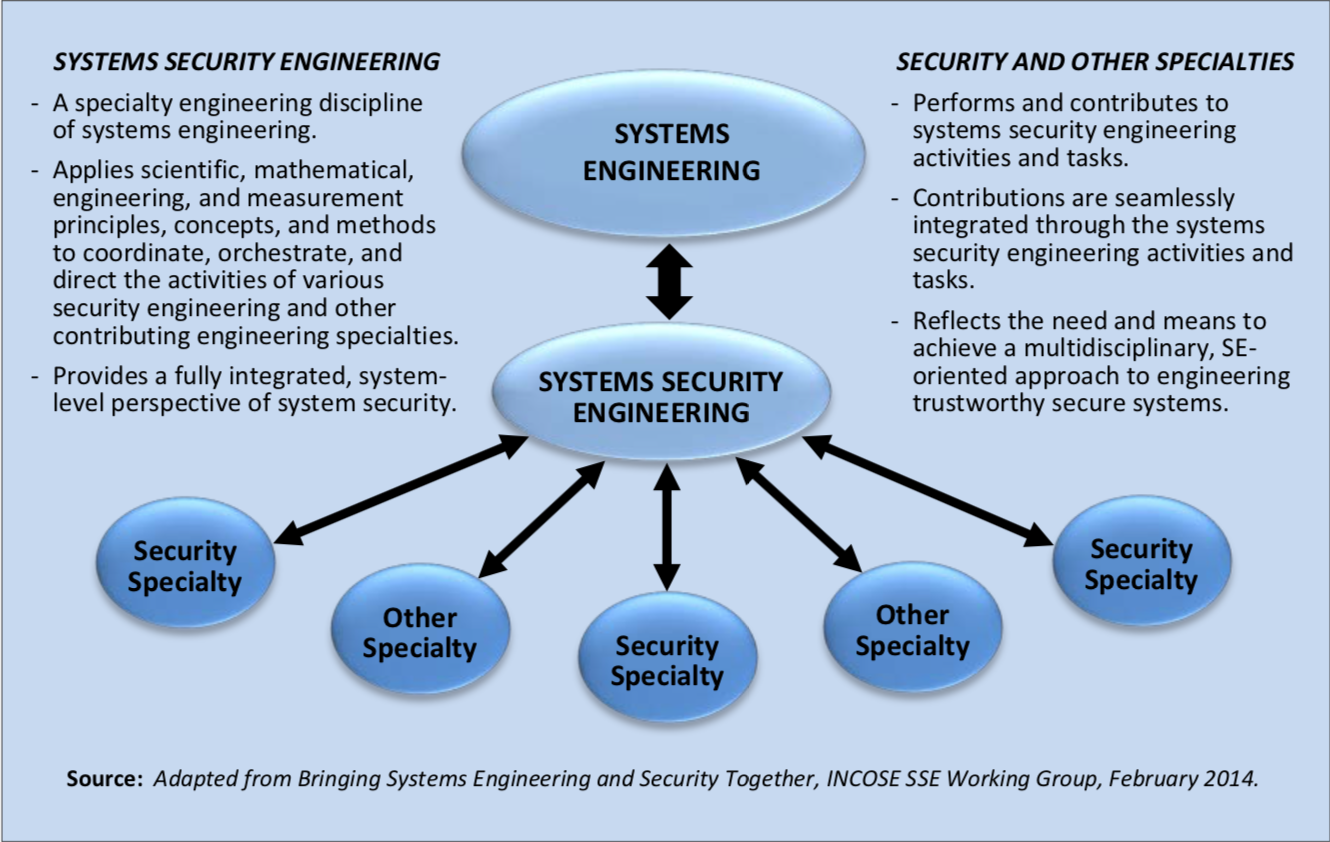
\includegraphics[width=\linewidth]{../figures/seincontext.png}
\caption{This is a clip from NIST 800-160.}
\label{fig:nist800160}
\end{figure}

This is some text after the figure.

\subsection{Trustworthiness}\label{ssec:trustworthiness}
\subsubsection{Complete Mediation}\label{sssec:completemediation}

\subsection{Verification}\label{ssec:verification}
\subsection{Documentation}\label{ssec:documentation}
\subsection{Reproducibility}\label{ssec:reproducibility}

      %%%%%%%%%%%%%%%%%%% Section Verification & Documentation %%%%%%
\section{Verification \& Documentation}

      %%%%%%%%%%%%%%%%%%% Section Complete Mediation %%%%%%%%%%%
\section{Principle of Complete Mediation}

\subsection{Formal Verification Using Computer-Aided Reasoning}

\end{document}